% First manuscript draft. Experimental values are generated from data/*.json.
\documentclass[a4paper,runningheads,twocolumn]{llncs}
% Two-column reading layout for the English draft only.
\usepackage[a4paper,margin=20mm,headheight=14pt,headsep=7mm]{geometry}
\usepackage{adjustbox}
\setlength{\columnsep}{7mm}
\setlength{\dbltextfloatsep}{12pt plus 2pt minus 2pt}
\setlength{\textfloatsep}{10pt plus 2pt minus 2pt}
\renewcommand{\dbltopfraction}{0.9}
\renewcommand{\textfraction}{0.08}
\renewcommand{\floatpagefraction}{0.75}
\renewcommand{\dblfloatpagefraction}{0.75}
\setcounter{dbltopnumber}{3}

\usepackage[T1]{fontenc}
\usepackage{lmodern}
\usepackage{amsmath,amssymb,bm}
\usepackage{graphicx,booktabs}
\usepackage{tikz}
\usetikzlibrary{arrows.meta,positioning}
\usepackage{xurl}
\usepackage[hidelinks]{hyperref}
\hypersetup{pdftitle={Robust Visual-Inertial Odometry with Linear Time-Varying Observer-Aided Constraints},pdfauthor={liuhe},pdfsubject={First manuscript draft},pdfkeywords={VIO, LTV Observer, ESKF, MSCKF}}
\newcommand{\R}{\mathbb{R}}
\newcommand{\sk}[1]{[#1]_{\times}}
\newcommand{\diag}{\operatorname{diag}}
\newcommand{\tr}{\operatorname{tr}}
\newcommand{\Exp}{\operatorname{Exp}}
\newcommand{\norm}[1]{\left\lVert #1\right\rVert}
\newcommand{\placeholder}[1]{\par\smallskip\noindent\textit{[Figure placeholder: #1]}\par\smallskip}
\emergencystretch=1em

\begin{document}
\title{Robust Visual-Inertial Odometry with Linear Time-Varying Observer-Aided Constraints}
\titlerunning{LTV Observer-Aided Visual-Inertial Odometry}
\author{liuhe}
\authorrunning{liuhe}
\institute{Huazhong University of Science and Technology, Wuhan, China\\
\email{liuhe2024@hust.edu.cn}}
\twocolumn[
\begin{@twocolumnfalse}
\maketitle

\begin{abstract}
Visual-inertial odometry combines camera observations with inertial measurements to estimate motion, yet the contribution of additional motion constraints depends on their formulation and fusion strength. This paper investigates a linear time-varying (LTV) observer as an auxiliary estimator for a multi-state constraint Kalman filter. Body-frame gravity, velocity, and landmark estimates are converted into three error-state measurement models. Gravity is constrained on a two-dimensional tangent plane, velocity couples attitude and world-frame velocity, and landmark constraints connect the current pose with a historical pose clone. Valid auxiliary blocks are assembled with visual residuals using a common prior and applied in one Kalman update. A bounded feature interface and a per-frame landmark information budget control the auxiliary supply. On ten EuRoC sequences, frozen scene- and mode-specific configurations are evaluated using trajectory error, relative motion error, local windows, update counts, and serial runtime measurements. Velocity and full fusion reduce position ATE on all four evaluated Machine Hall sequences, with mean relative reductions of 7.410\% and 7.578\%, respectively, while Vicon changes remain small. The measured computational overhead is substantial, identifying an important implementation trade-off.
\keywords{Visual-inertial odometry \and Linear time-varying observer \and Error-state Kalman filter \and Auxiliary constraints}
\end{abstract}
\vspace{6mm}
\end{@twocolumnfalse}
]

\section{Introduction}
Reliable motion estimation is essential for autonomous robots operating without an external positioning system. Cameras provide geometric constraints, while an inertial measurement unit (IMU) supplies high-rate rotational and translational motion information. Their complementary characteristics motivate visual-inertial odometry (VIO). Nevertheless, motion estimation remains sensitive to the available feature geometry, motion excitation, inertial bias, and the relative strength of the fused constraints.

Filter-based VIO maintains a motion state and its uncertainty while using image observations to correct inertial propagation. The stereo multi-state constraint Kalman filter (S-MSCKF) uses historical camera poses to obtain visual constraints without retaining every feature as a persistent filter state~\cite{sun2018}. OpenVINS provides a modular implementation of this approach, including first-estimate Jacobians (FEJ), calibrated sensor models, and flexible state management~\cite{geneva2020}. These systems are suitable platforms for studying auxiliary measurements because new residual blocks can be related directly to existing error-state variables.

A complementary perspective is to formulate motion quantities in the moving body frame. Wang and Tayebi~\cite{wang2024} introduce an LTV observer that estimates body-frame landmark positions, velocity, and gravity from inertial inputs and bearing observations. This representation avoids including attitude explicitly in the corresponding linear state. It suggests an opportunity to use these estimated quantities as auxiliary constraints within an established VIO estimator, while retaining the latter's inertial bias estimation and multi-view visual update.

The practical question is how to translate these outputs into usable error-state constraints. A gravity vector should constrain its direction without adding an artificial magnitude measurement. A body-frame velocity observation depends jointly on attitude and world-frame velocity. A landmark estimate requires a consistent temporal anchor and coordinate transformation. In addition, measurements computed at one prior must not be submitted after that prior has changed. These considerations motivate the unified fusion interface developed here.

We study three branches, denoted G, V, and L, and their full combination GVL. The implementation uses the existing stereo frontend and an LTV side estimator; it does not introduce an additional sensor or an external map. Experiments on EuRoC~\cite{burri2016} examine both the accuracy benefit and the cost of this integration. The remainder of the paper presents the theoretical preliminaries, the fusion method, the experiments, and the conclusions. The main contributions are:
\begin{enumerate}
\item An LTV observer-aided measurement formulation for gravity direction, body-frame velocity, and temporally anchored landmark position, with Jacobians matched to the VIO error convention.
\item A unified update interface that assembles visual and accepted auxiliary residuals at a common prior, together with bounded feature management, branch validity checks, and a landmark information budget.
\item A reproducible five-mode evaluation with frozen scene-specific configurations, reporting full-trajectory and local errors, actual auxiliary use, and serial computational overhead.
\end{enumerate}

\section{Theoretical Preliminaries}
\subsection{Frames, Inertial Inputs, and Bearing Geometry}
Let $\{W\}$, $\{B\}$, and $\{C\}$ denote the world, IMU body, and camera frames. We use $R\in SO(3)$ to map world-frame vectors into the body frame. Position $p$ and velocity $v$ are expressed in $\{W\}$, and $g_W=[0,0,-g]^\top$ is physical gravity. For $u\in\R^3$, $\sk{u}$ satisfies $\sk{u}w=u\times w$. Hats denote estimates and superscripts $-$ and $+$ denote prior and posterior quantities.

With calibrated, bias-corrected IMU inputs $\omega$ and $a$, the nominal kinematics are
\begin{equation}
 \dot R=-\sk{\omega}R,\qquad
 \dot p=v,\qquad
 \dot v=R^\top a+g_W .
 \label{eq:kinematics}
\end{equation}
Here $a$ is specific force, not acceleration with gravity already removed. Bias correction is applied once, using the current VIO bias estimates and the fixed sensor calibration.

Let $R_{BC}$ map camera vectors into the body frame, and let $p_{BC}$ be the camera center expressed in the body frame. For a static world point $P_i$, define its body-frame position
\begin{equation}
 \ell_i=R(P_i-p),\qquad
 P_i^C=R_{BC}^{\top}(\ell_i-p_{BC}).
 \label{eq:pointframes}
\end{equation}
A calibrated image coordinate yields the unit bearing
\begin{equation}
 b_i=\frac{[u_i^{n},v_i^{n},1]^\top}
 {\norm{[u_i^{n},v_i^{n},1]^\top}},\qquad d_i=R_{BC}b_i .
\end{equation}
The projection $\Pi_i=I_3-d_id_i^\top$ removes the unknown depth and gives the linear relation
\begin{equation}
 y_i=\Pi_i p_{BC}=\Pi_i\ell_i .
 \label{eq:bearing}
\end{equation}
All camera extrinsics and timestamps are transformed into the same body-frame convention before constructing observer inputs.
\placeholder{World, IMU body, and camera frames; camera offset $p_{BC}$, unit bearing $b_i$, and body-frame landmark $\ell_i$.}

\subsection{Body-Frame LTV Observer}
Following the body-frame formulation in~\cite{wang2024}, introduce $v_B=Rv$ and $\eta=Rg_W$. Their dynamics, together with those of the static landmarks, are
\begin{equation}
 \begin{aligned}
 \dot\ell_i&=-\sk{\omega}\ell_i-v_B,\\
 \dot v_B&=-\sk{\omega}v_B+\eta+a,\\
 \dot\eta&=-\sk{\omega}\eta .
 \end{aligned}
 \label{eq:ltvdynamics}
\end{equation}
For $N$ managed landmarks, let
\begin{equation}
 \begin{gathered}
 z=[\ell_1^\top,\ldots,\ell_N^\top,v_B^\top,\eta^\top]^\top,\\
 \dot z=Az+Ba,\quad y=Cz .
 \end{gathered}
 \label{eq:ltvstate}
\end{equation}
Writing $\Omega_N=\diag(\sk{\omega},\ldots,\sk{\omega})$ and
$\Gamma=\bm{1}_N\otimes I_3$, the matrices are
\begin{equation}
 \begin{gathered}
 A=\begin{bmatrix}
 -\Omega_N&-\Gamma&0\\
 0&-\sk{\omega}&I_3\\
 0&0&-\sk{\omega}
 \end{bmatrix},\\
 B=\begin{bmatrix}0\\I_3\\0\end{bmatrix},\quad
 C=\begin{bmatrix}\diag(\Pi_1,\ldots,\Pi_N)&0&0\end{bmatrix}.
 \end{gathered}
 \label{eq:ltvmatrices}
\end{equation}
Only currently observed landmarks contribute rows to $C$. The observer and its Riccati weighting matrix $P_L$ satisfy
\begin{align}
 \dot{\hat z}&=A\hat z+Ba+K_L(y-C\hat z),\label{eq:observer}\\
 K_L&=P_LC^\top Q_L, \notag\\
 \dot P_L&=AP_L+P_LA^\top-P_LC^\top Q_LCP_L+V_L .
 \label{eq:riccati}
\end{align}
The positive design matrices $Q_L$ and $V_L$ control correction and regularization. We use the landmark, velocity, and gravity outputs of this observer; the separate nonlinear pose observer of~\cite{wang2024} is not part of the proposed fusion.

The implementation propagates between IMU samples and applies bearing correction at image events. Forward Euler steps are used for the LTV state and Riccati terms, with bounded correction substeps. Feature birth and retirement resize the landmark blocks while retaining the surviving blocks and the velocity/gravity state. These operations are distinct from adding SLAM landmarks to the main VIO filter.

\subsection{Error-State Filtering and MSCKF Visual Constraints}
The VIO state contains the current inertial state and historical IMU pose clones:
\begin{equation}
 \begin{aligned}
 x&=(R,p,v,b_g,b_a,x_{c_1},\ldots,x_{c_M}),\\
 \delta x_I&=[\delta\theta^\top,\delta p^\top,\delta v^\top,
              \delta b_g^\top,\delta b_a^\top]^\top .
 \end{aligned}
\end{equation}
Our attitude error is defined by
\begin{equation}
 R_{\mathrm{true}}=\Exp(-\sk{\delta\theta})\hat R
       \simeq (I_3-\sk{\delta\theta})\hat R .
 \label{eq:attitudeerror}
\end{equation}
Vector errors are additive. The corresponding linearized inertial model is
$\delta\dot x_I=F\delta x_I+Gn_I$. Discretization gives the transition $\Phi_k$ and integrated process noise $Q_k$, so
\begin{equation}
 P_{I,k+1}^-=\Phi_kP_{I,k}^+\Phi_k^\top+Q_k .
 \label{eq:covprop}
\end{equation}
Cross-covariances with the clones are propagated consistently. At an image event, the current pose is cloned through its augmentation Jacobian. This retains the correlations needed for multi-view constraints~\cite{sun2018,geneva2020}.

For a feature observed at several poses, linearization yields
\begin{equation}
 r_f=H_x\delta x+H_f\delta P_f+n_f .
\end{equation}
An orthonormal left-nullspace basis $U$ with $U^\top H_f=0$ eliminates the feature error:
\begin{equation}
 r_{\mathrm{vis}}=U^\top r_f,\qquad
 H_{\mathrm{vis}}=U^\top H_x,\qquad
 R_{\mathrm{vis}}=U^\top R_fU .
 \label{eq:msckf}
\end{equation}
Accepted feature blocks are stacked and compressed before the EKF update. FEJ evaluates the required Jacobians at stored first estimates, while residuals use the current state. In our experiments, calibration is fixed and native SLAM landmarks are disabled. Features are still tracked and triangulated for MSCKF constraints.

\section{LTV Observer-Aided ESKF Fusion}
\subsection{Common-Prior Fusion Interface}
Figure~\ref{fig:framework} shows the integration. The IMU adapter advances the observer to the image time, using bracketed samples and the calibrated bias-corrected inputs. The feature interface supplies tracked bearings and geometric initialization. The observer produces $\hat\eta$, $\hat v_B$, and $\hat\ell_i$, while the main filter supplies its prior state, covariance, and live pose clones.

\begin{figure*}[t]
\centering
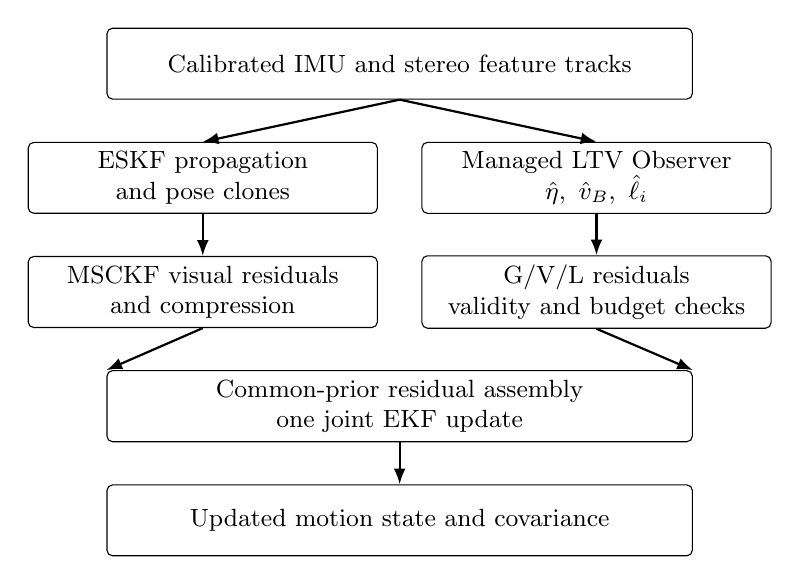
\begin{tikzpicture}[font=\small,
 box/.style={draw,rounded corners=2pt,align=center,minimum height=9mm,text width=42mm},
 flow/.style={-{Latex[length=2mm]},thick}]
\node[box,text width=72mm] (input) at (0,0) {Calibrated IMU and stereo feature tracks};
\node[box] (vio) at (-2.5,-1.45) {ESKF propagation\\and pose clones};
\node[box] (ltv) at (2.5,-1.45) {Managed LTV Observer\\$\hat\eta,\ \hat v_B,\ \hat\ell_i$};
\node[box] (vis) at (-2.5,-2.9) {MSCKF visual residuals\\and compression};
\node[box] (aux) at (2.5,-2.9) {G/V/L residuals\\validity and budget checks};
\node[box,text width=72mm] (joint) at (0,-4.35) {Common-prior residual assembly\\one joint EKF update};
\node[box,text width=72mm] (out) at (0,-5.8) {Updated motion state and covariance};
\draw[flow] (input.south) -- (vio.north);
\draw[flow] (input.south) -- (ltv.north);
\draw[flow] (vio) -- (vis);
\draw[flow] (ltv) -- (aux);
\draw[flow] (vis.south) -- (joint.north west);
\draw[flow] (aux.south) -- (joint.north east);
\draw[flow] (joint) -- (out);
\end{tikzpicture}
\caption{LTV observer-aided VIO. Geometric seeds, inertial biases, and the common filter prior are supplied through the integration interface. Auxiliary branches may be rejected individually.}
\label{fig:framework}
\end{figure*}

Each auxiliary block is described by $(r_j,H_j,R_j)$ and an ordered set of state variables. Jacobian columns are mapped into the native filter state without duplicating shared variables. A frame record identifies the image time, corresponding IMU time, observer epoch, and sequence number. Before submission, the implementation verifies that the main prior, its FEJ values, covariance, and clone set still match the values used to construct the block. An accepted record is consumed once.

For all branches, we use the residual convention $r=z_{\mathrm{aux}}-h(\hat x)$ and the linearized equation $r\simeq H\delta x+n$. Thus $H$ is the derivative of the prediction $h$, rather than the derivative of the fixed-measurement residual. Below, a superscript $f$ denotes the FEJ linearization value; residuals are evaluated at the current prior.

\subsection{Gravity Direction Constraint}
Let $\gamma=g_W/\norm{g_W}$ and $u_L=\hat\eta/\norm{\hat\eta}$. Select an orthonormal basis $T\in\R^{3\times2}$ for the tangent plane orthogonal to $d^f=R^f\gamma$, so $T^\top d^f=0$. Keeping this basis fixed during linearization gives
\begin{equation}
 r_G=T^\top(u_L-\hat R\gamma),\qquad
 H_{G,\theta}=T^\top\sk{R^f\gamma}.
 \label{eq:gravity}
\end{equation}
All other direct Jacobian blocks are zero. The two-dimensional residual constrains direction and avoids treating the observer's gravity magnitude as an additional observation. Its effective covariance is
\begin{equation}
 R_G=\sigma_G^2I_2,\qquad
 \sigma_G=\frac{\sigma_{G,0}}{\sqrt{\alpha_G}},
 \label{eq:gnoise}
\end{equation}
with angles converted to radians. The evaluated base value is $\sigma_{G,0}=10^\circ$. Increasing $\alpha_G$ changes information weighting; it does not directly multiply the Kalman gain.

\subsection{Body-Frame Velocity Constraint}
The observer velocity is compared with the main world-frame velocity transformed into the body frame:
\begin{equation}
 r_V=\hat v_B-\hat R\hat v,\qquad
 H_V=\begin{bmatrix}
 \sk{R^fv^f}&0&R^f&0&0&0_{\mathrm{clones}}
 \end{bmatrix}.
 \label{eq:velocity}
\end{equation}
The attitude and velocity columns are both necessary. For example, changing attitude while holding $v$ fixed changes the predicted body-frame velocity. We use
\begin{equation}
 R_V=\sigma_V^2I_3,\qquad
 \sigma_V=\frac{\sigma_{V,0}}{\sqrt{\alpha_V}},\qquad
 \sigma_{V,0}=1~\mathrm{m/s}.
 \label{eq:vnoise}
\end{equation}
Corrections can also affect position and inertial biases through the main filter's cross-covariances, although these variables do not appear directly in $H_V$.

\subsection{Temporally Anchored Landmark Constraint}
For a tracked landmark $i$, store its observer position $\hat\ell_{i,a}$ at a historical image time $t_a$ whose IMU pose clone remains in the filter. Given the current pose $(R_t,p_t)$ and anchor pose $(R_a,p_a)$, its predicted current body-frame position is
\begin{equation}
 \begin{aligned}
 h_{L,i}(x)&=R_t\big(R_a^\top\hat\ell_{i,a}+p_a-p_t\big),\\
 r_{L,i}&=\hat\ell_{i,t}^{-}-h_{L,i}(\hat x).
 \end{aligned}
 \label{eq:landmark}
\end{equation}
Here $\hat\ell_{i,t}^{-}$ is captured after observer inertial propagation and before the current bearing correction. The historical anchor is a stored post-camera observer snapshot. Both landmark estimates remain fixed when differentiating the main-state prediction. For the local column order $[\delta\theta_t,\delta p_t,\delta\theta_a,\delta p_a]$, the prediction Jacobian is
\begin{equation}
 H_{L,i}=
 \begin{bmatrix}
 \sk{h_{L,i}^f}&-R_t^f&
 -R_t^f(R_a^f)^\top\sk{\hat\ell_{i,a}}&R_t^f
 \end{bmatrix}.
 \label{eq:landmarkH}
\end{equation}
This branch constrains relative pose geometry. It neither treats $\hat\ell_{i,a}$ as a known world landmark nor adds the observer landmarks to the main ESKF state.

To obtain bounded and reproducible auxiliary supply, a candidate must be mature, velocity-ready, associated with a live anchor, and geometrically valid. The frozen implementation requires
\begin{equation}
 \begin{gathered}
 0.20\leq t-t_a\leq0.55~\mathrm{s},\\
 \frac{\norm{\hat\ell_{i,t}^{-}-h_{L,i}(\hat x)}}
 {\max(\norm{h_{L,i}(\hat x)},0.1~\mathrm{m})}\leq0.02 .
 \end{gathered}
 \label{eq:lvalid}
\end{equation}
Positive camera depth and feature association are checked. Candidates are selected deterministically, with at most $m_{\max}=2$ points per frame.

The landmark branch uses a range- and age-dependent effective variance,
\begin{align}
 s_{i,0}^2&=\big(\sigma_{L,\min}+0.02\norm{\hat\ell_{i,t}^{-}}\big)^2
       \left(1+\frac{t-t_a}{0.55~\mathrm{s}}\right),\\
 q_i&=\tr(H_{L,i}P_i^-H_{L,i}^{\top}),\notag\\
 s_i^2&=\max\left(s_{i,0}^2,\frac{q_i}{\beta_L/m_{\max}}\right),\notag\\
 R_{L,i}&=s_i^2 I_3 .
 \label{eq:lbudget}
\end{align}
$P_i^-$ is the marginal main covariance for the current and anchor pose blocks. The cap ensures $q_i/s_i^2\leq\beta_L/m_{\max}$. The variance is modified before computing the Kalman gain; the resulting state correction is not clipped afterward. The base setting is $\sigma_{L,\min}=0.5$ m and $\beta_L=0.01$. At landmark strength $\alpha_L$, these become $0.5/\sqrt{\alpha_L}$ m and $0.01\alpha_L$, respectively. This is an effective weighting rule, not a substitution of the observer Riccati matrix for measurement noise.

\subsection{Validity Checks and Joint Update}
The observer feature pool is bounded to 30 landmarks, with a minimum of 15 for its configured operation and 20 healthy image corrections for initial warmup. Seeds are obtained from stereo geometry when available, followed by temporal geometry. Feature identities include the observer epoch and birth information, preventing a retired track or reused identifier from being associated with an old anchor.

Auxiliary submission requires timestamp agreement within $10^{-6}$ s, a valid observer snapshot, branch readiness, finite state values, and a positive-definite innovation covariance. Gravity additionally requires $\norm{\hat\eta}\in[7,12]$ m/s$^2$ and at most $30^\circ$ directional disagreement. G and V are gated separately using normalized innovation squared:
\begin{equation}
 \nu_j=r_j^\top(H_jP^-H_j^\top+R_j)^{-1}r_j\leq\tau_j ,
 \label{eq:nis}
\end{equation}
where $\tau_G=9.21034$ and $\tau_V=11.34487$, corresponding to 99\% chi-square thresholds for two and three residual dimensions. The landmark branch uses the eligibility and information-budget rules above. The evaluated configuration does not enable the optional Huber reweighting.

After visual compression and branch selection, the accepted blocks are assembled as
\begin{equation}
 \begin{gathered}
 r=\begin{bmatrix}r_{\mathrm{vis}}\\r_G\\r_V\\r_L\end{bmatrix},\qquad
 H=\begin{bmatrix}H_{\mathrm{vis}}\\H_G\\H_V\\H_L\end{bmatrix},\\
 R_{\mathrm{eff}}=\diag(R_{\mathrm{vis}},R_G,R_V,R_L).
 \end{gathered}
 \label{eq:joint}
\end{equation}
Disabled or rejected blocks are omitted. This block-diagonal effective noise model is the weighting approximation used by the implementation. All quantities are associated with one frozen main-filter prior. The joint update is
\begin{align}
 S&=HP^-H^\top+R_{\mathrm{eff}},\\
 K&=P^-H^\top S^{-1},\notag\\
 \delta\hat x&=Kr,\notag\\
 x^+&=x^-\boxplus\delta\hat x,\notag\\
 P^+&=P^--KSK^\top .
 \label{eq:ekf}
\end{align}
Linear systems are solved by Cholesky factorization rather than explicitly forming $S^{-1}$. The native manifold update applies the attitude correction according to~\eqref{eq:attitudeerror}. Shared state columns are included once, and the full main covariance supplies the corresponding cross-covariances. Visual measurement compression is completed before adding the mixed-unit auxiliary rows.

The per-image procedure is:
\begin{enumerate}
\item Propagate and clone the main state; advance the LTV observer to the same sensor time.
\item Capture eligible landmark predictions before current bearing correction, then update the managed observer with the current bearings.
\item Freeze the main prior, build G/V and anchored L blocks, and construct the accepted MSCKF visual residuals.
\item Align Jacobian columns, verify the frame record and prior, and apply one joint EKF update. If auxiliary blocks are unavailable, retain the native visual update.
\item Archive post-camera landmark snapshots for live anchors and record which branches were actually applied.
\end{enumerate}

\section{Experiments}
\subsection{Dataset, Baseline, and Frozen Protocol}
We evaluate the method on ten EuRoC MAV sequences~\cite{burri2016}. The set comprises four Machine Hall runs (MH\_01, MH\_02, MH\_03, and MH\_05) and six Vicon runs (V1\_01--V1\_03 and V2\_01--V2\_03). MH\_04 was excluded before this final experiment because the baseline had diverged; its outcome is retained as an excluded baseline failure rather than counted as a successful sequence.

The baseline OFF is pure OpenVINS with the LTV observer disabled. G, V, and L activate the corresponding auxiliary branch, and GVL activates all three. Every mode uses stereo tracking, fixed calibration, FEJ, RK4 main-state integration, 11 pose clones, at most 40 MSCKF features per update, and no native SLAM landmarks or zero-velocity updates. The auxiliary LTV parameters are identical across all ON modes: $Q_L=10^{-4}I$, $V_L=10^6I$, and initial $P_L=I$ for the configured blocks.

Table~\ref{tab:weights} specifies the final information weights. Machine Hall and Vicon use different frozen profiles, and a single profile is used for every sequence within a scene category. The sequences had already been used for parameter selection; this evaluation is a frozen configuration confirmation. Because branch weights differ between single-branch and combined modes, the five-mode table is a tuned configuration comparison.
\begin{table}[tb]
\caption{Frozen scene- and mode-specific information weights. OFF disables the observer and every auxiliary branch.}\label{tab:weights}
\centering\small
\begin{tabular}{llrrr}
\toprule
Scene & Mode & $\alpha_G$ & $\alpha_V$ & $\alpha_L$ \\
\midrule
MH & G & 16 & -- & -- \\
MH & V & -- & 49 & -- \\
MH & L & -- & -- & 6 \\
MH & GVL & 2 & 49 & 6 \\
Vicon & G & 1 & -- & -- \\
Vicon & V & -- & 6 & -- \\
Vicon & L & -- & -- & 6 \\
Vicon & GVL & 1 & 1 & 1 \\
\bottomrule
\end{tabular}
\end{table}


The archived implementation identifies source revision \texttt{5ce89b93}, and the frozen data and protocol are available in the experiment repository~\cite{experiment2026}. We use 50 newly executed full-input accuracy runs and 50 separate serial resource measurements. The accuracy runs may be scheduled concurrently, but their runtime is not used for performance comparison. All 50 serial trajectories match their corresponding accuracy trajectories byte for byte in the archive.

ATE is position RMSE after $SE(3)$ alignment without scale. Each ON run is evaluated on the complete matched support fixed by its OFF run. Matched ground-truth coverage among estimated output rows ranges from 98.756\% to 99.612\%; OFF support coverage is 100\% for every evaluated configuration. This percentage does not include the pre-initialization segment as estimated output.

We also compute body-relative translation and rotation RPE at 1 and 5 s, with a 25 ms endpoint-matching tolerance. Local position RMSE uses fixed 10 s windows and the full-trajectory alignment, without realigning each window. The final 10\% of matched support is evaluated separately from the P95/P99 error distribution. The corrected orientation-ground-truth provenance for V1\_01 has not been verified, so its attitude-dependent RPE is descriptive only.

\subsection{Trajectory Accuracy and Scene Dependence}
Table~\ref{tab:ate} gives the full position ATE results, and Table~\ref{tab:summary} reports mean per-sequence relative reductions. All 50 configurations completed with finite output, identical initialization timing, and full baseline support in the archived evaluation.
\begin{table}[tb]
\caption{Position ATE RMSE (m) after rigid alignment without scale. Bold denotes the minimum in each row; very small differences are not interpreted as significant gains.}\label{tab:ate}
\centering\small
\begin{tabular}{lrrrrr}
\toprule
Sequence & OFF & G & V & L & GVL \\
\midrule
MH\_01 & 0.185425 & 0.183850 & \textbf{0.182746} & 0.185464 & 0.182761 \\
MH\_02 & 0.097130 & 0.096057 & 0.086545 & 0.096256 & \textbf{0.085925} \\
MH\_03 & 0.149282 & 0.148537 & 0.136360 & 0.149006 & \textbf{0.136077} \\
MH\_05 & 0.276242 & 0.276290 & \textbf{0.252370} & 0.276371 & 0.252777 \\
V1\_01 & 0.064243 & 0.064241 & 0.064249 & \textbf{0.064225} & 0.064238 \\
V1\_02 & 0.068188 & 0.068192 & 0.068201 & \textbf{0.068183} & 0.068193 \\
V1\_03 & 0.041891 & 0.041892 & \textbf{0.041890} & 0.041890 & 0.041891 \\
V2\_01 & 0.174581 & 0.174566 & \textbf{0.174542} & 0.174581 & 0.174559 \\
V2\_02 & 0.051975 & 0.051978 & \textbf{0.051967} & 0.051972 & 0.051976 \\
V2\_03 & 0.207428 & 0.207245 & \textbf{0.207228} & 0.207256 & 0.207248 \\
\bottomrule
\end{tabular}
\end{table}

\begin{table}[tb]
\caption{Mean per-sequence relative ATE reduction (\%). Positive is improvement; each sequence receives equal weight.}\label{tab:summary}
\centering\small
\begin{adjustbox}{max width=\columnwidth}
\begin{tabular}{lrrrr}
\toprule
Mode & MH (4) & Vicon (6) & All (10) & Lower ATE \\
\midrule
G & 0.609 & 0.014 & 0.252 & 6/10 \\
V & 7.410 & 0.018 & 2.975 & 8/10 \\
L & 0.254 & 0.021 & 0.114 & 7/10 \\
GVL & 7.578 & 0.016 & 3.041 & 7/10 \\
\bottomrule
\end{tabular}
\end{adjustbox}
\end{table}


The main improvement occurs in Machine Hall. V lowers ATE on all four evaluated MH sequences, with a mean relative reduction of 7.410\%. GVL also improves all four, with a mean reduction of 7.578\%. Its largest reduction is 11.535\% on MH\_02; reductions on MH\_03 and MH\_05 are 8.846\% and 8.494\%. V reduces MH\_05 ATE from 0.276242 m to 0.252370 m, a decrease of about 23.873 mm.

G produces smaller MH improvements, and L has mixed results. Their mean MH reductions are 0.609\% and 0.254\%, respectively. GVL outperforms V in ATE on MH\_02 and MH\_03, but V is slightly better on MH\_01 and MH\_05. Thus velocity is the dominant source of the observed accuracy benefit, and the full combination is not uniformly better than V alone.

Vicon changes are small. Mean relative reductions for all modes remain below 0.021\%, and the largest Vicon increase in V is about 0.0134 mm on V1\_02. These numerical changes support describing the position ATE as largely unchanged, rather than emphasizing small rankings. Across all ten sequences, V and GVL have mean relative ATE reductions of 2.975\% and 3.041\%, respectively.

\placeholder{Aligned OFF/V/GVL trajectories and position-error curves for MH\_02 and MH\_05, using the exact frozen matched support.}

\subsection{Relative Motion and Local Error}
Table~\ref{tab:mhmetrics} examines whether the ATE improvements are accompanied by changes in relative motion and error extremes. GVL lowers 1 s and 5 s translation RPE, final-support position RMSE, and maximum position error on all four evaluated MH sequences. On MH\_02, the final-support RMSE reduction is 21.48\%, and the maximum aligned position error reduction is 33.01\%. These measurements provide complementary evidence to full-trajectory ATE.
\begin{table}[tb]
\caption{Relative error reductions of GVL against OFF in Machine Hall (\%). Tail is position RMSE over the final 10\% of matched support; max is the maximum aligned position error.}\label{tab:mhmetrics}
\centering\small
\begin{adjustbox}{max width=\columnwidth}
\begin{tabular}{lrrrrr}
\toprule
Sequence & ATE & RPE-T 1 s & RPE-T 5 s & Tail & Max \\
\midrule
MH\_01 & 1.44 & 4.61 & 1.83 & 2.85 & 0.30 \\
MH\_02 & 11.54 & 8.88 & 5.92 & 21.48 & 33.01 \\
MH\_03 & 8.85 & 2.31 & 2.43 & 11.07 & 6.95 \\
MH\_05 & 8.49 & 2.31 & 1.47 & 8.48 & 6.34 \\
\bottomrule
\end{tabular}
\end{adjustbox}
\end{table}


Overall improvements do not imply that every local interval improves. In the fixed 10 s analysis, the largest relative GVL increase is 9.018\% (3.368 mm) in MH\_03 window index 5. V increases the same window by 8.552\% (3.193 mm). The largest absolute GVL window increase is about 5.821 mm in V2\_03 window index 11. G has a maximum relative local increase of 6.081\% (2.754 mm) in MH\_01 window index 7. These outcomes are reported alongside the gains rather than hidden by a trajectory-level average.
\placeholder{Fixed-window position RMSE comparison for OFF, V, and GVL, including the local increases on MH\_03 and V2\_03.}

\subsection{Actual Auxiliary Use and Computational Cost}
Table~\ref{tab:updates} reports the frames in which each GVL branch was actually applied. Nonzero application counts on every evaluated sequence distinguish active fusion from merely enabling a configuration flag. Different counts are expected because landmark maturity, live anchors, and gravity/velocity readiness are separate checks.
\begin{table}[tb]
\caption{Frames with actually applied auxiliary branches in GVL. Counts can differ because each branch has its own validity conditions.}\label{tab:updates}
\centering\small
\begin{tabular}{lrrr}
\toprule
Sequence & G & V & L \\
\midrule
MH\_01 & 2350 & 2343 & 2343 \\
MH\_02 & 1499 & 1478 & 1478 \\
MH\_03 & 2078 & 1929 & 1927 \\
MH\_05 & 1638 & 1578 & 1578 \\
V1\_01 & 2426 & 2407 & 2406 \\
V1\_02 & 953 & 932 & 930 \\
V1\_03 & 956 & 931 & 927 \\
V2\_01 & 1574 & 1563 & 1560 \\
V2\_02 & 1606 & 1571 & 1570 \\
V2\_03 & 706 & 637 & 627 \\
\bottomrule
\end{tabular}
\end{table}


Resource measurements use complete serial input replays, an exclusive performance lock, the same two-logical-CPU affinity, a verified single OpenCV thread, and the same diagnostic level. Mode order alternates forward and reverse by sequence. The table aggregates paired increases by first computing each sequence's percentage change against OFF and then taking the median.
\begin{table}[tb]
\caption{Median per-sequence increases over OFF (\%). Camera P95 measures only the camera API; full-run CPU and wall time include the complete replay. One serial paired measurement per sequence and mode.}\label{tab:cost}
\centering\small
\begin{adjustbox}{max width=\columnwidth}
\begin{tabular}{lrrrr}
\toprule
Mode & Camera P95 & CPU time & Wall time & Peak RSS \\
\midrule
G & +337.14 & +214.81 & +214.88 & +22.94 \\
V & +335.27 & +214.46 & +214.61 & +22.74 \\
L & +341.14 & +218.42 & +218.65 & +22.92 \\
GVL & +340.78 & +219.22 & +219.40 & +21.69 \\
\bottomrule
\end{tabular}
\end{adjustbox}
\end{table}


GVL increases median full-run CPU time by 219.22\%, corresponding to approximately 3.19 times the OFF CPU time. Its camera API P95 increases by 340.78\%, while peak resident memory increases by 21.69\%. The absolute GVL camera P95 values range from about 27.07 to 44.68 ms in this measured environment. The camera API does not include the complete IMU and input/output processing path; full-run measurements are therefore reported separately.

Only one paired serial measurement is available for each sequence and mode, so these timings are descriptive measurements without independent timing confidence intervals. The measured ON camera P95 and peak-memory increases exceed the archive's historical 5\% and 10\% overhead limits in every pair. These outcomes concern computational cost and do not invalidate the separately measured trajectory improvements.

\subsection{Discussion}
The experiment identifies a useful operating regime for the velocity-aided branch in Machine Hall, while the Vicon profiles preserve nearly the same full-trajectory position accuracy. The different scene responses motivate reporting both categories instead of relying only on a single overall mean. They also motivate evaluating a fixed parameter-selection rule on sequences not used for tuning in future work.

The modest additional benefit of G/L means that enabling every branch should be justified by the application and its error metrics. The landmark branch participates in many updates, yet its standalone ATE benefit is small; application count is evidence of execution, not a guarantee of benefit. Moreover, the mode-dependent weights mean that these results do not isolate all pairwise interactions among the three branches.

The current implementation has a substantial resource cost. Similar measured costs across G, V, L, and GVL suggest that profiling the common observer and integration path is a useful next step, although the present measurements do not attribute runtime to individual internal operations. The method should consequently be evaluated as an accuracy--cost trade-off rather than presented as a lightweight enhancement.

\section{Conclusion}
This paper presents an LTV observer-aided fusion method for a filter-based visual-inertial estimator. Body-frame gravity direction, velocity, and temporally anchored landmark position are expressed as error-state residuals, with matched Jacobians, branch validity checks, and a bounded landmark information budget. Accepted auxiliary blocks and visual constraints are applied in one common-prior Kalman update.

Frozen configuration confirmation on ten EuRoC sequences shows that velocity and full GVL fusion reduce ATE on all four evaluated Machine Hall sequences. GVL obtains a mean MH reduction of 7.578\%, accompanied by lower translation RPE and final-support errors. Vicon position ATE remains largely unchanged, and some local windows increase despite overall gains. The CPU and camera-latency overhead is substantial. Future work will focus on profiling and reducing this overhead, evaluating frozen configurations on independent sequences, and examining when each auxiliary branch provides an application-relevant benefit.

\bibliographystyle{splncs04}
\bibliography{references}
\end{document}
